%\section{Discussion}
%In this section, we first evaluate importance of each relational view for our boosted model. We then compare with approaches proposed to merge neural networks in general in other domains. Finally, we study robustness of our model to training label sparsity.

%\vspace{-0.1in}
\subsection{Ablation Study on Relation Types}
\begin{table}[h]
  \vspace{-0.0in}
  \small
  %\robustify\bfseries
  \begin{tabular}{l | S[round-mode=places,round-precision=2]@{\hspace{2mm}}|S[round-mode=places,round-precision=2]@{\hspace{2mm}}|S[round-mode=places,round-precision=2]@{\hspace{2mm}}| S[round-mode=places,round-precision=2]@{\hspace{2mm}}|S[round-mode=places,round-precision=2]}
  %\begin{tabular}{l | c | c| c| c|c}
    \toprule
  %  \textbf{Strategies} &
      % \textbf{SF} &
      % \textbf{ENG} &
      % \textbf{SCIFI} &
      % \textbf{PHYS}&
      % \textbf{WP}\\
       \textbf{\{ Relation Type\}} &
        \textbf{Tech} &
        \textbf{Culture} &
        \textbf{Life} &
        \textbf{Sci}&
        \textbf{Business}\\
      \midrule
      C & 71.23 &75.90 &78.71&72.99 & 76.85\\
    \{ TS, AS \} & 67.86 &74.15 &75.75&65.80& 76.13  \\
    R & 68.30 & 73.35 & 76.57 & 67.40 & 75.76 \\
    \{TS, AS \} + R & 69.28 & 75.50 &76.41 &70.11  &77.90 \\
    C + R & 73.04 & 77.66 & 80.25 &73.72 & 80.04 \\
    C + \{ TS, AS \} & 72.81 & 78.04 & 81.41 & 72.19 & 80.15\\
    C + \{ TS, AS \} + R & \bfseries 73.87 & \bfseries 78.74 & \bfseries 81.60&  \bfseries74.68&  \bfseries80.56 \\
    \bottomrule
  \end{tabular}
  \caption{\small \label{tab:relation} 5-fold Accuracy (in \%) comparison for different combination of relation types for our boosted model. Contrastive and Similarity by Contrast relations together performs similar to the final model.}
  \vspace{-0.15in}
\end{table}

We present the results of an ablation study with a different combination of relation types (Contrastive, Similarity, and Reflexive) used for the IR-GCN model in Table \ref{tab:relation}. We conducted this study on the biggest community from each of the five categories, i.e., ServerFault (Technology), English (Culture), Science Fiction (Life), Physics (Science), Workplace (Business).
Similarity by Contrast relation (TrueSkill and Arrival) used in isolation performs the worst among all the variants. Training Contrastive and Similarity by Contrast relation together in our boosted framework performs similar to our final model. Reflexive GCN contributes the least as it does not consider any neighbors.

\vspace{-0.1in}
\subsection{Aggregator Architecture Variants}
\label{sec:agg}
We compare our gradient boosting based aggregation approach with other popular methods used in literature to merge different neural networks discussed in \cref{item:aggregator}.

\begin{table}[h]
  \small
  %\robustify\bfseries
  \vspace{-0.15in}
  \begin{tabular}{l | c | c| c| c|c}
    \toprule
    % \textbf{Method} &
    %   \textbf{SF} &
    %   \textbf{ENG} &
    %   \textbf{SCIFI} &
    %   \textbf{PHYS}&
    %   \textbf{WP}\\
    \textbf{Method} &
     \textbf{Tech} &
     \textbf{Culture} &
     \textbf{Life} &
     \textbf{Sci}&
     \textbf{Business}\\
      \midrule
    Stacking~\cite{Stacking} &68.58 & 74.44 & 79.19 & 70.29 &75.50  \\
    Fusion~\cite{Fusion18}  &72.30 &77.25 & 80.79 & 73.91 &79.01 \\
    NeighborAgg~\cite{graphsage,relationalGCN}  &69.29 &74.28 & 77.94 & 68.42 &78.64   \\
    IR-GCN & \bfseries 73.87 & \bfseries 78.74 & \bfseries 81.60&  \bfseries74.78&  \bfseries80.56 \\
    \bottomrule
  \end{tabular}
  \caption{\small \label{tab:agg} 5-fold Accuracy (in \%) comparison of different aggregator architectures. These architectures perform worse than Contrastive GCN. Fusion performs similarly but is computationally expensive.}
  \vspace{-0.2in}
\end{table}

Table \ref{tab:agg} reports the accuracy results for these aggregator variants as compared to our model. Our method outperforms all the variants with Fusion performing the best. This worse performance reaffirms that existing aggregation models are not suitable for our problem. Note that these approaches perform worse than even Contrastive GCN except Fusion. The fusion approach performs similarly to our approach but is computationally expensive as the input size for each IR-GCN in fusion is linear in the number of all views in the model.

\subsection{Textual Features}
Most of the current literature focuses on using textual features for Answer Selection. In this section, we compare our proposed IR-GCN model to a popular text-based model~\cite{Tan2015}. %proposed for answer selection.

\noindent
\textbf{QA-LSTM/CNN \cite{Tan2015}} uses a stacked bidirectional LSTM model followed by convolution filters to learn embeddings for the question and answer text separately. They then rank answers in decreasing order of the cosine similarity between question and answer embeddings.

  %\item{\textbf{biLSTM+CNN} The basic biLSTM model was extended to learn more composite embedding by using convolution filters on biLSTM output.}
\noindent
\textbf{Textual Similarity (T-GCN)} We create a \textit{Similarity by Contrast} view that connects answers authored by a user where her answer's text is significantly similar (dissimilar) to the question's text than the other competing answers. We used cosine similarity on the learned question and answer embeddings from the QA-LSTM approach as the similarity function.

\noindent
\textbf{IR-GCN + T-GCN} extends our proposed model to also include the Textual Similarity as the third \textit{Similarity by Contrast} view in addition to Arrival and TrueSkill views.
\begin{table}[h]
  \small
  %\robustify\bfseries
  \centering
    \vspace{-0.0in}
  \begin{tabular}{l | S[round-mode=places,round-precision=2]S[round-mode=places,round-precision=2]S[round-mode=places,round-precision=2]S[round-mode=places,round-precision=2]S[round-mode=places,round-precision=2]}
    \toprule
    \textbf{Method} &
      \textbf{Tech} &
      \textbf{Culture} &
      \textbf{Life} &
      \textbf{Sci} &
      \textbf{Business}\\
      \midrule
    QA-LSTM/CNN\cite{Tan2015} & 66.49 & 71.70 & 69.42 & 62.91 & 72.55 \\
    FF~\cite{JendersKN16} & 68.30 & 73.35 & 76.57 & 67.40 & 75.76 \\
    T-GCN & 69.25 & 73.77 & 76.39 & 67.79 & 77.08\\
    IR-GCN & 73.87 & 78.74 & 81.60 & 74.68 & 80.56 \\
    IR-GCN + T-GCN & 73.89 & 78.00  & 81.07 & 74.49 & 78.86\\
    \bottomrule
  \end{tabular}
  \caption{\small \label{tab:text} 5-fold Accuracy comparison of text-based baseline and textual similarity GCN with IR-GCN.}
    \vspace{-0.2in}
\end{table}

In general, the text-based baseline, QA-LSTM, performs worse than even reflexive GCN, as shown in Table \ref{tab:text}. Note that reflexive GCN employs a feedforward model on the activity and user features used in our experiments. This is a surprising result as most of the current literature focus on textual features for the task. Our results indicate that non-textual features are useful too for the answer selection task on StackExchange communities.

Textual Similarity GCN performs better than QA-LSTM and Reflexive GCN. Even though we use the output of QA-LSTM to construct the graph for T-GCN, the graph improves performance as it connects answers across different questions. However, adding the T-GCN view in our proposed IR-GCN model decreases the performance slightly. One possible explanation could be that similarity by contrast views based on user features (Arrival similarity and TrueSkill similarity) are not compatible with views based on textual features.

% \begin{table}[h]
%   \small
%   %\robustify\bfseries
%   \centering
%   \begin{tabular}{l | S[round-mode=places,round-precision=2]S[round-mode=places,round-precision=2]S[round-mode=places,round-precision=2]S[round-mode=places,round-precision=2]S[round-mode=places,round-precision=2]}
%     \toprule
%     \textbf{Method} &
%       \textbf{Tech} &
%       \textbf{Culture} &
%       \textbf{Life} &
%       \textbf{Sci} &
%       \textbf{Business}\\
%       \midrule
%     QA-LSTM/CNN\cite{Tan2015} & 66.49 &  & 69.42 & 62.91 & 72.55 \\
%     FF~\cite{JendersKN16} & 66.00 & 72.22 & 69.85 & 63.63 & 75.57 \\
%     CS-GCN & 66.06 & 72.35 & 71.88 & 64.14 & 75.69 \\
%     IR-GCN & 66.56 & 72.92 & 72.54 & 65.11 & 75.95 \\
%     IR-GCN + CS-GCN & 66.49 & 73.17 & 72.85 & 65.29 & 75.86 \\
%     \bottomrule
%   \end{tabular}
%   \caption{\small \label{tab:textfeature} 5-fold Accuracy comparison of content-based baseline and content-similarity GCN with learnt content embeddings as features in the GCN.}
% \end{table}
%
% We further replaced our activity based features with the learned embeddings obtained after training the QA-LSTM/CNN~\cite{Tan2015} model. We observed that performance of all approaches went down slightly when using content features (Table \ref{tab:textfeature}). As we noted before, GCNs aggregate features among the neighbors. In our similar contrast view, it is not favorable to aggregate content features among the neighbors as we connect answers catering to different questions. Thus, aggregating content features will create noise in the dataset.

\vspace{-0.2in}
\subsection{Discriminative Magnification effect}

% \begin{figure}[tbh]
%   \centering
%   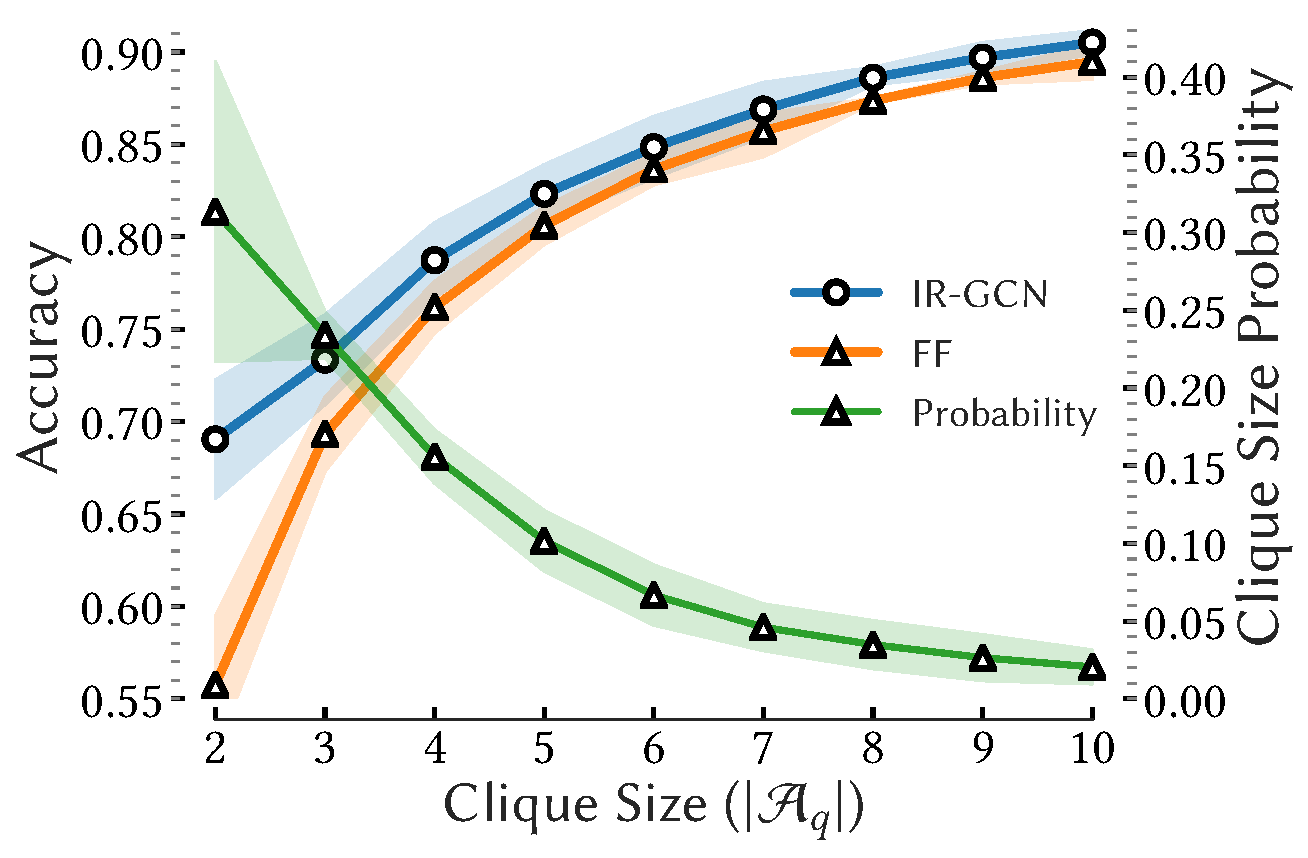
\includegraphics[scale=0.3]{figures/clique_acc.pdf}
%   %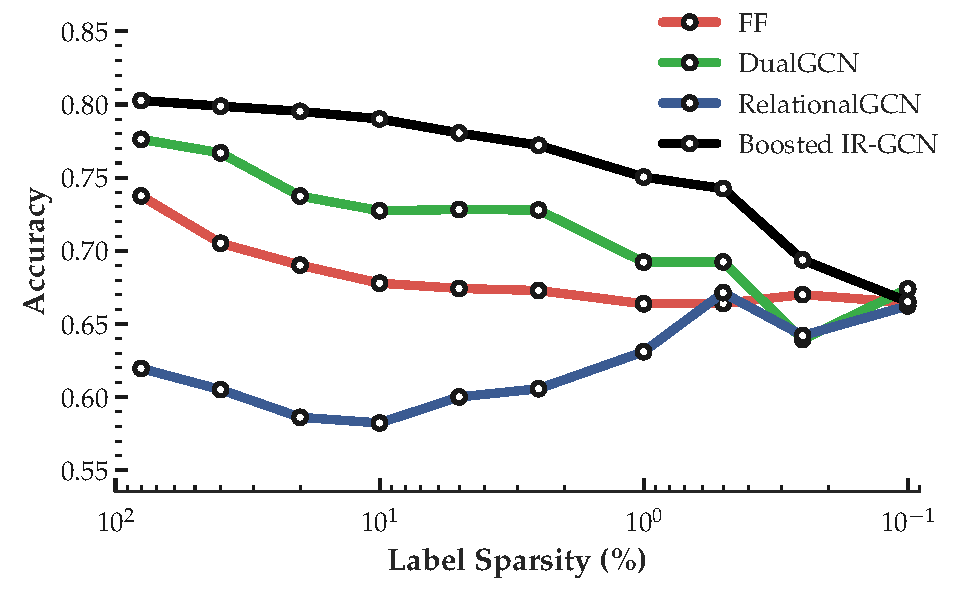
\includegraphics[height=4.2cm,width=0.85\linewidth]{figures/Label_Sparsity}
%   \vspace{-0.12in}
%   \caption{\small \label{fig:clique} Accuracy of our IR-GCN model compared to the FF model with varying clique size (i.e. number of answers to a question, $\vert \mathcal{A}_q \vert$) for Contrastive view . %The results are reported for the largest StackExchange community in all five categories.
% We report averaged results over the largest community of all categories. Our model performs much better for smaller cliques, and the effect diminishes for larger cliques (\cref{eq:contrast}). 80\% of the questions have $< 4$ answers.}
%   \vspace{-0.15in}
% \end{figure}

We show that due to our proposed modification to the convolution operation for contrastive view, we achieve \emph{Discriminative Magnification effect} (\cref{eq:contrast}). Note that the difference is scaled by Clique size ($1 + 1/n-1$), i.e. number of answers to a question, $\vert \mathcal{A}_q \vert$. Figure \ref{fig:clique} shows the accuracy of our IR-GCN model as compared to the FeedForward model with varying clique size. Recall that the FeedForward model predict node labels independent of other nodes and is not affected by clique size. We report average results over the same five communities as above. We can observe that increase in accuracy is much more for lower clique sizes (13\% improvement for $\vert \mathcal{A}_q \vert = 2$ and 4\% for $\vert \mathcal{A}_q \vert = 3$ on average). The results are almost similar for larger clique sizes. In other words, our model significantly outperforms the FeedForward model for questions with fewer candidate answers. However, around 80\% of the questions have very few answers($< 4$), and thus this gain over FF is significant.

\vspace{-0.2in}
\subsection{Label Sparsity}

\begin{figure}[tbh]
  \begin{subfigure}{0.4\textwidth}
    \centering
    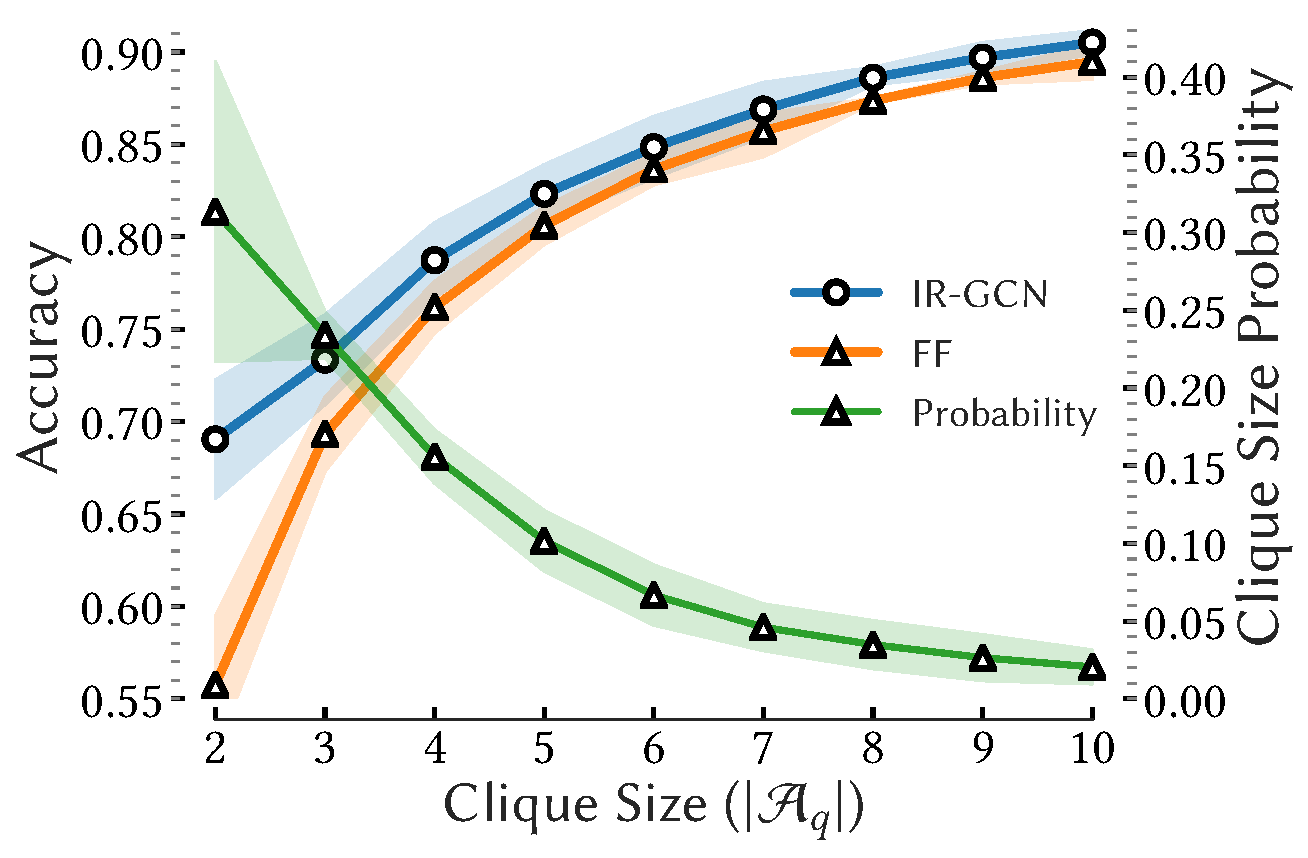
\includegraphics[scale=0.26]{figures/clique_acc.pdf}
    %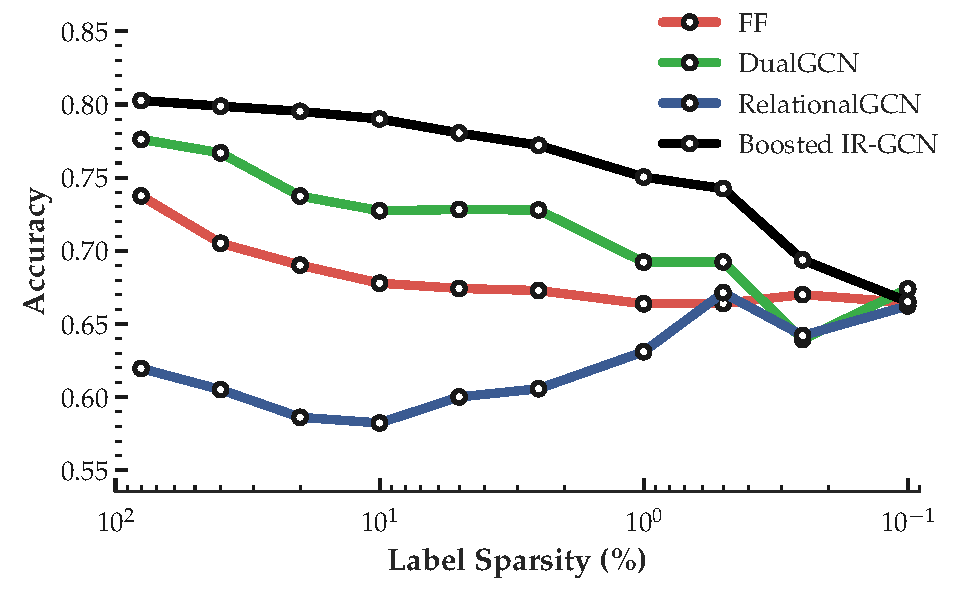
\includegraphics[height=4.2cm,width=0.85\linewidth]{figures/Label_Sparsity}
    \caption{\small \label{fig:clique}}
    %\vspace{-0.12in}
  \end{subfigure} \hspace{0.3in}
  \begin{subfigure}{0.55\textwidth}
      \centering
  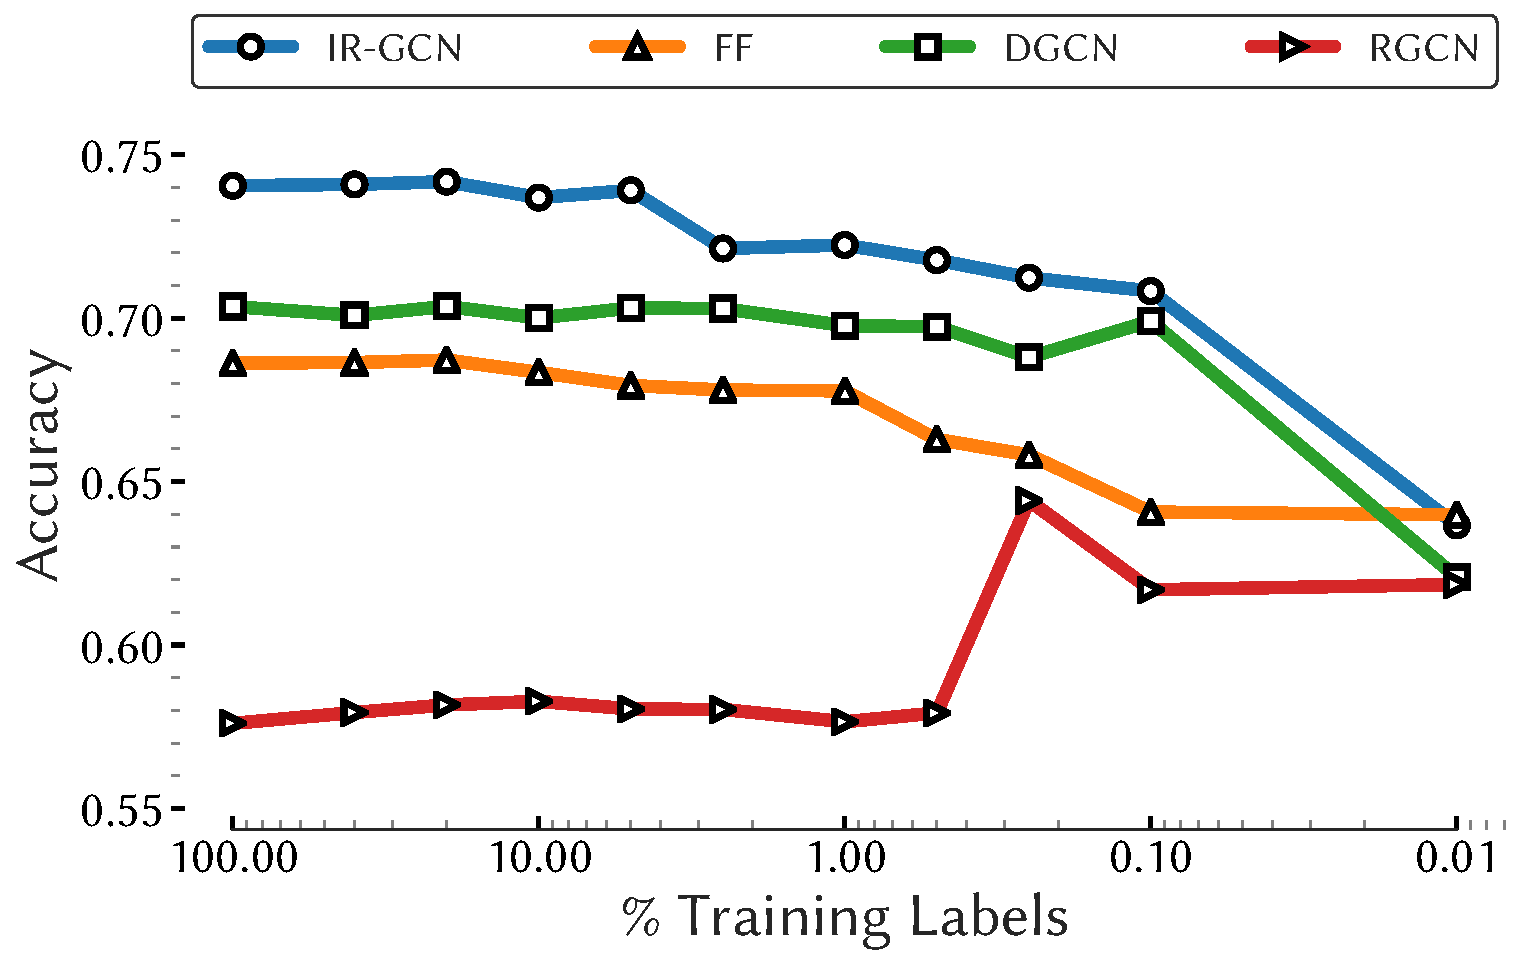
\includegraphics[scale=0.25]{figures/sparsity_acc_physics.pdf}
  %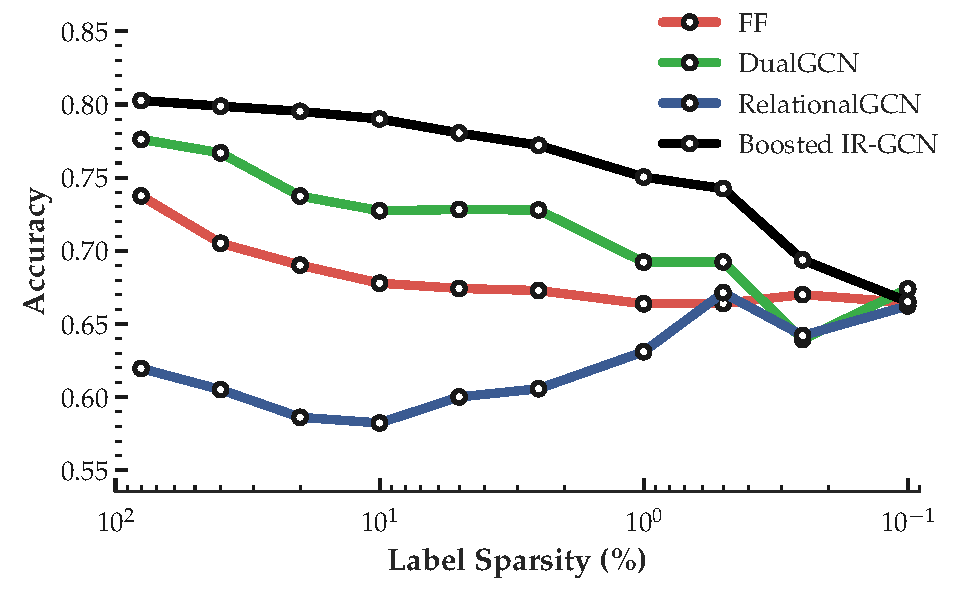
\includegraphics[height=4.2cm,width=0.85\linewidth]{figures/Label_Sparsity}
  %\vspace{-0.2in}
  \caption{\small\label{fig:labelsparsity} }
  \end{subfigure}
  %\vspace{-0.2in}
  \caption{\small a) Accuracy of our IR-GCN model compared to the FF model with varying clique size (i.e., number of answers to a question, $\vert \mathcal{A}_q \vert$) for Contrastive view. %The results are reported for the largest StackExchange community in all five categories.
We report averaged results over the largest community of all categories. Our model performs much better for smaller cliques, and the effect diminishes for larger cliques (\cref{eq:contrast}). 80\% of the questions have $< 4$ answers. \\
b) Change in accuracy with varying training label rates for Physics StackExchange. Our model is more robust to label sparsity than other relation ensemble approaches. RGCN works better with fewer labels as contrastive relation introduces noise in the model. At extreme sparsity, all approaches converge to the same value indicating random selection.
}
\end{figure}
Graph Convolution Networks are robust to label sparsity as they exploit graph structure and are thus heavily used for semi-supervised settings. Figure \ref{fig:labelsparsity} shows the change in accuracy for Physics StackExchange from the Science category at different training label rates. Even though our graph contains disconnected cliques, IR-GCN still preserves robustness to label sparsity.
In contrast, the accuracy of the FeedForward model declines sharply with less label information. Performance of DualGCN remains relatively stable while Relational GCN's performance increases with a decrease in label rate. Relational GCN assumes each view to be of similarity relation, and thus, adding contrastive relation introduces noise in the model. However, as the training labels become extremely sparse, the training noise decreases that leads to a marked improvement in the model. In the case of a meager label rate of 0.01\%, all approaches converge to the same value, which is the expectation of theoretically random selection. We obtained similar results for the other four StackExchange communities but omitted them for brevity.

% \subsection{Change in Accuracy with Clique Size}

\begin{comment}
\subsection{Contrastive GCN Analysis}
\label{ref:analysis}
The ability of neural networks to perform classification in sparse high-dimensional manifolds has been studied in past work, especially in the context of adversarial learning \cite{lu2017safetynet}. We employ the ReLU activation function in our convolution layers and study the outputs of the $k$th layer, i.e. embeddings with k-order locality. This transformation breaks the input space into cells with smooth gradients within each cell, at whose boundaries the piecewise linear function changes (i.e. the likelihood of the two classes of answers).

% In the context of adversarial learning \cite{safetynet} propose the existence of p-domains or cells in the learned manifold, representing a piecewise linear mapping of the transformed features to the class labels. The generalization neutrality property is particularly interesting. Both train and test samples are highly unlikely to lie in p-domains since the number of examples is much smaller than the capacity of the neural network to fit these regions. Weight decay can incentivize relatively small changes in the gradient across these regions resulting in smoother changes.  the ability of the network to fit such regions in the data manifold?

We ask a specific question in the context of our Contrastive IR-GCN. \emph{What is the impact of the layerwise discriminative magnification induced by our formulation?} Discriminative magnifications results in improved separability of the two classes in the later convolving layers, an effect we earlier demonstrated with a sample network in \cref{fig:contrast}. This positively impacts the ability of the model to explain the observed data points (i.e create p-domains that are well aligned with the contrastive samples provided) and improve the generalizability of the learned model to unseen data points. However, it is important to maintain sufficient regularization with weight decay to prevent sparse regions exhibiting sharp gradients which could affect model performance.

The capacity of our model can also be quantified in terms of the VC dimension of the aggregated classifier against the individual learners. Gradient boosting with multiple relation learners (each of which captures a specific aspect of node locality via graph convolution on the induced relations) could boost the capacity of the joint model, enabling better generalization and a more accurate fit in the data manifold (i.e. higher capacity to fit regions to fine distinctions).

Let us denote the upper bound of the VC dimension or capacity of each individual learner as D (If the individual learners do not have identical capacity, the minimum can be used to compute a lower bound on the aggregated learner capacity). Then the gradient boosted learner with T classifiers has a bound on it's capacity~\cite{shalev2014understanding} given by,
\begin{equation*}
\mathcal{VC}_{Agg}  = T \times (D+1) \times(3 \log(T.(D+1))+2)
\label{vcdim}
\vspace{-0.03in}
\end{equation*}

Thus we identify two potential reasons for our performance gains, first the discriminative magnification effect which also supports the strong individual performance of the contrast view, and second the gain in capacity from boosting, which could explain it's advantage over competing aggregation methods.

\end{comment}
